\documentclass{article}
\usepackage{../cs170}
\usepackage{pgfplots}
\pgfplotsset{compat=1.18}
\AtBeginDocument{\RenewCommandCopy\qty\SI}

\def\title{HW 02}

\begin{document}

\maketitle

\question{}

\begin{center}
    \begin{circuitikz}
        \draw (0, 0) node[ground]{} to[sV, l=\(V_s\)] (0, 2) to[R, l=\(R\)] (2, 2) to[L, l=\(L\)] (2, 0) node[ground]{};
        \draw (2, 2) to[short] (3, 2) node[ocirc]{\(V_o\)}
    ;\end{circuitikz}
\end{center}

\begin{subparts}
    \item The differential equation governing the circuit is
    \begin{align}
        V_s(t) - I_L(t) R - L \dv{I_L}{t} &= 0 \\
        \implies \dv{I_L}{t} + \frac{R}{L} I_L(t) &= \frac{1}{L} V_s(t)
    \end{align}
    The homogeneous solution to the differential equation is
    \begin{equation}
        I_{L, h}(t) = A_h e^{-\frac{R}{L} t}
    \end{equation}
    Assuming the particular solution is of the form \(A_p e^{bt}\), we have
    \begin{equation}
        A_p be^{bt} + \frac{R}{L} A_p e^{bt} = \frac{1}{L} u(t)
    \end{equation}
    Pattern matching, we find that \(b = 0\), and \(A_p = \frac{1}{R} u(t)\), so our particular solution is
    \begin{equation}
        I_{L, p}(t) = \frac{1}{R} u(t)
    \end{equation}
    The final solution is
    \begin{align}
        I_L(t) &= I_{L, h}(t) + I_{L, p}(t) = \frac{1}{R} u(t) + A_h e^{-\frac{R}{L} t} \\
        I_L(0) &= 0 = \frac{1}{R} + A_h \implies A_h = -\frac{1}{R} u(t)
    \end{align}
    The final equation is
    \begin{align}
        I_L(t) &= \frac{1}{R} (1 - e^{-\frac{R}{L} t}) u(t) \\
        V_o(t) &= L \dv{I_L}{t} = \cancelto{0}{\frac{L}{R} (1 - e^{-\frac{R}{L} t}) \delta(t)} + e^{-\frac{R}{L} t} u(t)
    \end{align}
    The impulse response, by definition, is
    \begin{equation}
        h(t) = \dv{\Phi_o}{t} = \cancelto{1}{e^{-\frac{R}{L} t}} \delta(t) - \frac{R}{L} e^{-\frac{R}{L} t} u(t) = \delta(t) - \frac{R}{L} e^{-\frac{R}{L} t} u(t)
    \end{equation}
    Assuming \(V_s = \qty{1}{\volt}\), \(R = \qty{1}{\ohm}\), \(L = \qty{1}{\henry}\),
    \begin{center}
        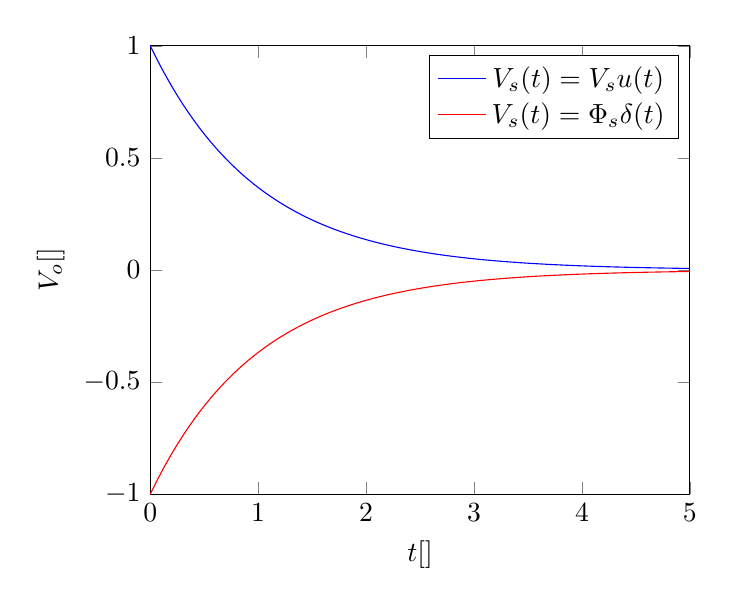
\begin{tikzpicture}
            \begin{axis}[
                xlabel = {\(t [\unit{\second}]\)},
                ylabel = {\(V_o [\unit{\volt}]\)},
                xmin = 0, xmax = 5,
                ymin = -1, ymax = 1,
            ]
                \addplot[
                domain = 0:5,
                samples = 100,
                color = blue
                ]
                {exp(-x)};
                \addlegendentry{\(V_s(t) = V_s u(t)\)}

                \addplot[
                domain = 0:5,
                samples = 100,
                color = red
                ]
                {-exp(-x)};
                \addlegendentry{\(V_s(t) = \Phi_s \delta(t)\)}
            \end{axis}
        \end{tikzpicture}
    \end{center}
    \item Finding the particular solution for the frequency response, we have
    \begin{equation}
        A be^{bt} + \frac{R}{L} A e^{bt} = \frac{1}{L} V_s e^{j \omega t}
    \end{equation}
    Pattern matching, we find that \(b = j \omega\), and \(A = \frac{V_s}{R + j \omega L}\).
    The final equation is
    \begin{align}
        I_L(t) &= \frac{V_s}{R + j \omega L} e^{j \omega t} \\
        V_o(t) &= L \dv{I_L}{t} = \frac{V_s L}{R + j \omega L} j \omega e^{j \omega t} \\
        &= \frac{V_s e^{j \omega t}}{R + j \omega L} (j \omega L) \implies \frac{V_o(t)}{V_s(t)} = \frac{j \omega L}{R + j \omega L} \\
        \left|\frac{V_o(t)}{V_s(t)}\right| &= \frac{\omega L}{\sqrt{R^2 + (\omega L)^2}} \\
        \angle \frac{V_o(t)}{V_s(t)} &= \tan^{-1}\left(\frac{R}{\omega L}\right)
    \end{align}
    This is a high-pass filter since \(\lim_{\omega \to 0} |H(\omega)| = 0\) and \(\lim_{\omega \to \infty} |H(\omega)| = 1\).
\end{subparts}

\question{}

\begin{subparts}
    \item \begin{equation}
        F(s) = \int_{\R^+} 7t^2 e^{-st} \, \dd{t}
    \end{equation}
    By tabular integration, we have
    \begin{equation}
        \begin{array}{c|c}
            u & v \\
            \hline
            7t^2 & e^{-st} \\
            14t & -\frac{1}{s} e^{-st} \\
            14 & \frac{1}{s^2} e^{-st} \\
            0 & -\frac{1}{s^3} e^{-st}
        \end{array}
    \end{equation}
    So the final integral is
    \begin{equation}
        F(s) = \eval{-\frac{7t^2 e^{-st}}{s} - \frac{14t e^{-st}}{s^2} - \frac{14 e^{-st}}{s^3}}_0^\infty = \frac{14}{s^3}
    \end{equation}
    where the integral converges when \(\Re\{s\} > 0\).
    \item \begin{align}
        F(s) &= \int_{\R^+} 3e^{-2t} \cos(5t) e^{-st} \, \dd{t} \\
        &= \int_{\R^+} 3e^{-2t} \left(\frac{e^{j 5t} + e^{-j 5t}}{2}\right) e^{-st} \, \dd{t} \\
        &= \frac{3}{2} \int_{\R^+} e^{(-2 - s + 5j) t} + e^{(-2 - s - 5j) t} \, \dd{t} \\
        &= \frac{3}{2} \left(\eval{\frac{1}{-2 - s + 5j} e^{(-2 - s + 5j) t} + \frac{1}{-2 - s - 5j} e^{(-2 - s - 5j) t}}_0^\infty\right) \\
        &= \frac{3}{2} \left(\frac{1}{2 + s + 5j} + \frac{1}{2 + s - 5j}\right) \\
        &= \frac{3}{2} \left(\frac{2 + s - 5j + 2 + s + 5j}{(2 + s)^2 + 25}\right) = 3 \left(\frac{2 + s}{(2 + s)^2 + 25}\right)
    \end{align}
    where the integral converges when \(\Re\{s\} > 2\).
\end{subparts}

\question{}

\begin{subparts}
    \item \begin{align}
        F(s) &= \frac{1}{s - 1} + \frac{4}{(s - 3)^2} + \frac{7}{(s - 5)^3} \\
        &= \frac{0!}{(s - 1)^1} + \frac{4}{1!} \frac{1!}{(s - 3)^2} + \frac{7}{2!} \frac{2!}{(s - 5)^3}
    \end{align}
    Using the Laplace transform pair \(t^n e^{-\alpha t} \iff \frac{n!}{(s + \alpha)^{n + 1}}\), we get
    \begin{equation}
        f(t) = e^t + 4t e^{3t} + \frac{7}{2} t^2 e^{5t}
    \end{equation}
    \item \begin{equation}
        F(s) = \frac{(s + 3) + 8}{(s + 3)^2 + 4} = \frac{s + 3}{(s + 3)^2 + 4} + 4 \frac{2}{(s + 3)^2 + 4}
    \end{equation}
    Using the Laplace transform pairs \(e^{-\alpha t} \sin(\omega t) \iff \frac{\omega}{(s + \alpha)^2 + \omega^2}\) and \(e^{-\alpha t} \cos(\omega t) \iff \frac{s + \alpha}{(s + \alpha)^2 + \omega^2}\), we get
    \begin{equation}
        f(t) = e^{-3t} \cos(2t) + 4e^{-3t} \sin(2t)
    \end{equation}
    \item \begin{align}
        F(s) &= \frac{1}{(s + 2) (s + 4)} = \frac{A}{s + 2} + \frac{B}{s + 4} \\
        \implies 1 &= A (s + 4) + B (s + 2)
    \end{align}
    Plugging in \(s = -4\) and \(s = -2\), we get \(A = \frac{1}{2}\) and \(B = -\frac{1}{2}\), respectively.
    We then get
    \begin{equation}
        F(s) = \frac{1}{2} \frac{1}{s + 2} - \frac{1}{2} \frac{1}{s + 4}
    \end{equation}
    Using the Laplace transform pair \(e^{-\alpha t} \iff \frac{1}{s + \alpha}\),
    \begin{equation}
        f(t) = \frac{1}{2} e^{-2t} - \frac{1}{2} e^{-4t}
    \end{equation}
\end{subparts}

\question{}

\begin{center}
    \begin{circuitikz}
        \draw (0, 0) node[ground]{} to[I, l=\(I_1 u(t)\)] (0, 2) to[short] (4, 2) to[R, l=\(R\)] (6, 2) to[V, l=\(V_1\)] (6, 0) node[ground]{};
        \draw (3, 2) to[I, l_=\(Q_1 \delta(t - t_0)\)] (3, 0) node[ground]{};
        \draw (4, 2) to[C, l=\(C\)] (4, 0) node[ground]{};
    \end{circuitikz}
\end{center}
Using superposition, we find \(V_c(t)\) considering only \(I_1 u(t)\):
\begin{center}
    \begin{circuitikz}
        \draw (0, 0) node[ground]{} to[I, l=\(I_1 u(t)\)] (0, 2) to[short] (4, 2) to[R, l=\(R\)] (6, 2) to[short] (6, 0) node[ground]{};
        \draw (4, 2) to[C, l=\(C\)] (4, 0) node[ground]{};
    \end{circuitikz}
\end{center}
The initial condition is \(V_c(0) = 0\).
The homogeneous solution is \(V_c(t) = A_h e^{-\frac{t}{RC}}\).
The particular solution governing the circuit is
\begin{align}
    \frac{I_1}{C} u(t) &= \dv{V_c}{t} + \frac{1}{RC} V_c(t) \\
    \frac{I_1}{C} u(t) &= A_p b e^{bt} + \frac{A_p}{RC} e^{bt} \\
    \implies V_c(t) &= I_1 R u(t) \\
    \implies V_c(t) &= I_1 R (1 - e^{-\frac{t}{RC}}) u(t)
\end{align}
Finding \(V_c(t)\) considering only \(Q_1 \delta(t - t_0)\):
\begin{center}
    \begin{circuitikz}
        \draw (3, 2) to[short] (4, 2);
        \draw (4, 2) to[R, l=\(R\)] (6, 2);
        \draw (6, 2) to[short] (6, 0) node[ground]{};
        \draw (3, 2) to[I, l_=\(Q_1 \delta(t - t_0)\)] (3, 0) node[ground]{};
        \draw (4, 2) to[C, l=\(c\)] (4, 0) node[ground]{};
    \end{circuitikz}
\end{center}
The initial condition is \(V_c(t_0) = 0\).
Taking the Laplace transform,
\begin{center}
    \begin{circuitikz}
        \draw (0, 0) node[ground]{} to[I, l=\(Q_1 e^{-t_0 s}\), invert] (0, 2) to[short] (2, 2) to[generic, l=\(Z\), a=\(\frac{R}{1 + sRC}\)] (2, 0) node[ground]{};
    \end{circuitikz}
\end{center}
By Ohm's law, we get
\begin{equation}
    V(s) = -\frac{QR e^{-t_0 s}}{\frac{1}{RC} + sRC} = -\frac{\frac
    {Q}{C} e^{-t_0 s}}{\frac{1}{RC} + s} \overset{\mathcal{L}^{-1}}{\implies} V_c(t) = -\frac{Q}{C} e^{-\frac{t - t_0}{RC}} u(t - t_0)
\end{equation}
% The homogeneous solution is \(V_c(t) = A_h e^{-\frac{t}{RC}}\).
% The particular solution governing the circuit is
% \begin{align}
%     -\frac{Q_1}{C} \delta(t - t_0) &= \dv{V_c}{t} + \frac{1}{RC} V_c(t) \\
%     -\frac{Q_1}{C} \delta(t - t_0) &= A_p b e^{bt} + \frac{A_p}{RC} e^{bt} \\
%     \implies V_c(t) &= -Q_1 R \delta(t - t_0) \\
%     \implies V_c(t) &= -Q_1 R (1 - e^{-\frac{t}{RC}}) \delta(t - t_0)
% \end{align}
Finding \(V_c(t)\) considering only \(V_1\):
\begin{center}
    \begin{circuitikz}
        \draw (4, 2) to[R, l=\(R\)] (6, 2) to[V, l=\(V_1\)] (6, 0) node[ground]{};
        \draw (4, 2) to[C, l=\(C\)] (4, 0) node[ground]{};
    \end{circuitikz}
\end{center}
Since \(V_1\) is a constant, \(V_c(t) = V_1\) is at steady state.
The final equation for the circuit is
\begin{equation}
    V_c(t) = I_1 R (1 - e^{-\frac{t}{RC}}) u(t) - \frac{Q}{C} e^{-\frac{t - t_0}{RC}} u(t - t_0) + V_1
\end{equation}
Assuming \(I_1 = \qty{1}{\ampere}\), \(Q_1 = \qty{1}{\coulomb}\), \(C = \qty{1}{\farad}\), \(R = \qty{1}{\ohm}\), \(V_1 = \qty{1}{\volt}\), and \(t_0 = \qty{2}{\second}\),
\begin{center}
    \resizebox{0.8\textwidth}{!}{%% Creator: Matplotlib, PGF backend
%%
%% To include the figure in your LaTeX document, write
%%   \input{<filename>.pgf}
%%
%% Make sure the required packages are loaded in your preamble
%%   \usepackage{pgf}
%%
%% Also ensure that all the required font packages are loaded; for instance,
%% the lmodern package is sometimes necessary when using math font.
%%   \usepackage{lmodern}
%%
%% Figures using additional raster images can only be included by \input if
%% they are in the same directory as the main LaTeX file. For loading figures
%% from other directories you can use the `import` package
%%   \usepackage{import}
%%
%% and then include the figures with
%%   \import{<path to file>}{<filename>.pgf}
%%
%% Matplotlib used the following preamble
%%   \usepackage{fontspec}
%%
\begingroup%
\makeatletter%
\begin{pgfpicture}%
\pgfpathrectangle{\pgfpointorigin}{\pgfqpoint{6.400000in}{4.800000in}}%
\pgfusepath{use as bounding box, clip}%
\begin{pgfscope}%
\pgfsetbuttcap%
\pgfsetmiterjoin%
\definecolor{currentfill}{rgb}{1.000000,1.000000,1.000000}%
\pgfsetfillcolor{currentfill}%
\pgfsetlinewidth{0.000000pt}%
\definecolor{currentstroke}{rgb}{1.000000,1.000000,1.000000}%
\pgfsetstrokecolor{currentstroke}%
\pgfsetdash{}{0pt}%
\pgfpathmoveto{\pgfqpoint{0.000000in}{0.000000in}}%
\pgfpathlineto{\pgfqpoint{6.400000in}{0.000000in}}%
\pgfpathlineto{\pgfqpoint{6.400000in}{4.800000in}}%
\pgfpathlineto{\pgfqpoint{0.000000in}{4.800000in}}%
\pgfpathlineto{\pgfqpoint{0.000000in}{0.000000in}}%
\pgfpathclose%
\pgfusepath{fill}%
\end{pgfscope}%
\begin{pgfscope}%
\pgfsetbuttcap%
\pgfsetmiterjoin%
\definecolor{currentfill}{rgb}{1.000000,1.000000,1.000000}%
\pgfsetfillcolor{currentfill}%
\pgfsetlinewidth{0.000000pt}%
\definecolor{currentstroke}{rgb}{0.000000,0.000000,0.000000}%
\pgfsetstrokecolor{currentstroke}%
\pgfsetstrokeopacity{0.000000}%
\pgfsetdash{}{0pt}%
\pgfpathmoveto{\pgfqpoint{0.800000in}{0.528000in}}%
\pgfpathlineto{\pgfqpoint{5.760000in}{0.528000in}}%
\pgfpathlineto{\pgfqpoint{5.760000in}{4.224000in}}%
\pgfpathlineto{\pgfqpoint{0.800000in}{4.224000in}}%
\pgfpathlineto{\pgfqpoint{0.800000in}{0.528000in}}%
\pgfpathclose%
\pgfusepath{fill}%
\end{pgfscope}%
\begin{pgfscope}%
\pgfsetbuttcap%
\pgfsetroundjoin%
\definecolor{currentfill}{rgb}{0.000000,0.000000,0.000000}%
\pgfsetfillcolor{currentfill}%
\pgfsetlinewidth{0.803000pt}%
\definecolor{currentstroke}{rgb}{0.000000,0.000000,0.000000}%
\pgfsetstrokecolor{currentstroke}%
\pgfsetdash{}{0pt}%
\pgfsys@defobject{currentmarker}{\pgfqpoint{0.000000in}{-0.048611in}}{\pgfqpoint{0.000000in}{0.000000in}}{%
\pgfpathmoveto{\pgfqpoint{0.000000in}{0.000000in}}%
\pgfpathlineto{\pgfqpoint{0.000000in}{-0.048611in}}%
\pgfusepath{stroke,fill}%
}%
\begin{pgfscope}%
\pgfsys@transformshift{1.025455in}{0.528000in}%
\pgfsys@useobject{currentmarker}{}%
\end{pgfscope}%
\end{pgfscope}%
\begin{pgfscope}%
\definecolor{textcolor}{rgb}{0.000000,0.000000,0.000000}%
\pgfsetstrokecolor{textcolor}%
\pgfsetfillcolor{textcolor}%
\pgftext[x=1.025455in,y=0.430778in,,top]{\color{textcolor}\rmfamily\fontsize{10.000000}{12.000000}\selectfont \(\displaystyle {0}\)}%
\end{pgfscope}%
\begin{pgfscope}%
\pgfsetbuttcap%
\pgfsetroundjoin%
\definecolor{currentfill}{rgb}{0.000000,0.000000,0.000000}%
\pgfsetfillcolor{currentfill}%
\pgfsetlinewidth{0.803000pt}%
\definecolor{currentstroke}{rgb}{0.000000,0.000000,0.000000}%
\pgfsetstrokecolor{currentstroke}%
\pgfsetdash{}{0pt}%
\pgfsys@defobject{currentmarker}{\pgfqpoint{0.000000in}{-0.048611in}}{\pgfqpoint{0.000000in}{0.000000in}}{%
\pgfpathmoveto{\pgfqpoint{0.000000in}{0.000000in}}%
\pgfpathlineto{\pgfqpoint{0.000000in}{-0.048611in}}%
\pgfusepath{stroke,fill}%
}%
\begin{pgfscope}%
\pgfsys@transformshift{1.927273in}{0.528000in}%
\pgfsys@useobject{currentmarker}{}%
\end{pgfscope}%
\end{pgfscope}%
\begin{pgfscope}%
\definecolor{textcolor}{rgb}{0.000000,0.000000,0.000000}%
\pgfsetstrokecolor{textcolor}%
\pgfsetfillcolor{textcolor}%
\pgftext[x=1.927273in,y=0.430778in,,top]{\color{textcolor}\rmfamily\fontsize{10.000000}{12.000000}\selectfont \(\displaystyle {2}\)}%
\end{pgfscope}%
\begin{pgfscope}%
\pgfsetbuttcap%
\pgfsetroundjoin%
\definecolor{currentfill}{rgb}{0.000000,0.000000,0.000000}%
\pgfsetfillcolor{currentfill}%
\pgfsetlinewidth{0.803000pt}%
\definecolor{currentstroke}{rgb}{0.000000,0.000000,0.000000}%
\pgfsetstrokecolor{currentstroke}%
\pgfsetdash{}{0pt}%
\pgfsys@defobject{currentmarker}{\pgfqpoint{0.000000in}{-0.048611in}}{\pgfqpoint{0.000000in}{0.000000in}}{%
\pgfpathmoveto{\pgfqpoint{0.000000in}{0.000000in}}%
\pgfpathlineto{\pgfqpoint{0.000000in}{-0.048611in}}%
\pgfusepath{stroke,fill}%
}%
\begin{pgfscope}%
\pgfsys@transformshift{2.829091in}{0.528000in}%
\pgfsys@useobject{currentmarker}{}%
\end{pgfscope}%
\end{pgfscope}%
\begin{pgfscope}%
\definecolor{textcolor}{rgb}{0.000000,0.000000,0.000000}%
\pgfsetstrokecolor{textcolor}%
\pgfsetfillcolor{textcolor}%
\pgftext[x=2.829091in,y=0.430778in,,top]{\color{textcolor}\rmfamily\fontsize{10.000000}{12.000000}\selectfont \(\displaystyle {4}\)}%
\end{pgfscope}%
\begin{pgfscope}%
\pgfsetbuttcap%
\pgfsetroundjoin%
\definecolor{currentfill}{rgb}{0.000000,0.000000,0.000000}%
\pgfsetfillcolor{currentfill}%
\pgfsetlinewidth{0.803000pt}%
\definecolor{currentstroke}{rgb}{0.000000,0.000000,0.000000}%
\pgfsetstrokecolor{currentstroke}%
\pgfsetdash{}{0pt}%
\pgfsys@defobject{currentmarker}{\pgfqpoint{0.000000in}{-0.048611in}}{\pgfqpoint{0.000000in}{0.000000in}}{%
\pgfpathmoveto{\pgfqpoint{0.000000in}{0.000000in}}%
\pgfpathlineto{\pgfqpoint{0.000000in}{-0.048611in}}%
\pgfusepath{stroke,fill}%
}%
\begin{pgfscope}%
\pgfsys@transformshift{3.730909in}{0.528000in}%
\pgfsys@useobject{currentmarker}{}%
\end{pgfscope}%
\end{pgfscope}%
\begin{pgfscope}%
\definecolor{textcolor}{rgb}{0.000000,0.000000,0.000000}%
\pgfsetstrokecolor{textcolor}%
\pgfsetfillcolor{textcolor}%
\pgftext[x=3.730909in,y=0.430778in,,top]{\color{textcolor}\rmfamily\fontsize{10.000000}{12.000000}\selectfont \(\displaystyle {6}\)}%
\end{pgfscope}%
\begin{pgfscope}%
\pgfsetbuttcap%
\pgfsetroundjoin%
\definecolor{currentfill}{rgb}{0.000000,0.000000,0.000000}%
\pgfsetfillcolor{currentfill}%
\pgfsetlinewidth{0.803000pt}%
\definecolor{currentstroke}{rgb}{0.000000,0.000000,0.000000}%
\pgfsetstrokecolor{currentstroke}%
\pgfsetdash{}{0pt}%
\pgfsys@defobject{currentmarker}{\pgfqpoint{0.000000in}{-0.048611in}}{\pgfqpoint{0.000000in}{0.000000in}}{%
\pgfpathmoveto{\pgfqpoint{0.000000in}{0.000000in}}%
\pgfpathlineto{\pgfqpoint{0.000000in}{-0.048611in}}%
\pgfusepath{stroke,fill}%
}%
\begin{pgfscope}%
\pgfsys@transformshift{4.632727in}{0.528000in}%
\pgfsys@useobject{currentmarker}{}%
\end{pgfscope}%
\end{pgfscope}%
\begin{pgfscope}%
\definecolor{textcolor}{rgb}{0.000000,0.000000,0.000000}%
\pgfsetstrokecolor{textcolor}%
\pgfsetfillcolor{textcolor}%
\pgftext[x=4.632727in,y=0.430778in,,top]{\color{textcolor}\rmfamily\fontsize{10.000000}{12.000000}\selectfont \(\displaystyle {8}\)}%
\end{pgfscope}%
\begin{pgfscope}%
\pgfsetbuttcap%
\pgfsetroundjoin%
\definecolor{currentfill}{rgb}{0.000000,0.000000,0.000000}%
\pgfsetfillcolor{currentfill}%
\pgfsetlinewidth{0.803000pt}%
\definecolor{currentstroke}{rgb}{0.000000,0.000000,0.000000}%
\pgfsetstrokecolor{currentstroke}%
\pgfsetdash{}{0pt}%
\pgfsys@defobject{currentmarker}{\pgfqpoint{0.000000in}{-0.048611in}}{\pgfqpoint{0.000000in}{0.000000in}}{%
\pgfpathmoveto{\pgfqpoint{0.000000in}{0.000000in}}%
\pgfpathlineto{\pgfqpoint{0.000000in}{-0.048611in}}%
\pgfusepath{stroke,fill}%
}%
\begin{pgfscope}%
\pgfsys@transformshift{5.534545in}{0.528000in}%
\pgfsys@useobject{currentmarker}{}%
\end{pgfscope}%
\end{pgfscope}%
\begin{pgfscope}%
\definecolor{textcolor}{rgb}{0.000000,0.000000,0.000000}%
\pgfsetstrokecolor{textcolor}%
\pgfsetfillcolor{textcolor}%
\pgftext[x=5.534545in,y=0.430778in,,top]{\color{textcolor}\rmfamily\fontsize{10.000000}{12.000000}\selectfont \(\displaystyle {10}\)}%
\end{pgfscope}%
\begin{pgfscope}%
\definecolor{textcolor}{rgb}{0.000000,0.000000,0.000000}%
\pgfsetstrokecolor{textcolor}%
\pgfsetfillcolor{textcolor}%
\pgftext[x=3.280000in,y=0.251889in,,top]{\color{textcolor}\rmfamily\fontsize{10.000000}{12.000000}\selectfont \(\displaystyle t\) [s]}%
\end{pgfscope}%
\begin{pgfscope}%
\pgfsetbuttcap%
\pgfsetroundjoin%
\definecolor{currentfill}{rgb}{0.000000,0.000000,0.000000}%
\pgfsetfillcolor{currentfill}%
\pgfsetlinewidth{0.803000pt}%
\definecolor{currentstroke}{rgb}{0.000000,0.000000,0.000000}%
\pgfsetstrokecolor{currentstroke}%
\pgfsetdash{}{0pt}%
\pgfsys@defobject{currentmarker}{\pgfqpoint{-0.048611in}{0.000000in}}{\pgfqpoint{-0.000000in}{0.000000in}}{%
\pgfpathmoveto{\pgfqpoint{-0.000000in}{0.000000in}}%
\pgfpathlineto{\pgfqpoint{-0.048611in}{0.000000in}}%
\pgfusepath{stroke,fill}%
}%
\begin{pgfscope}%
\pgfsys@transformshift{0.800000in}{1.084767in}%
\pgfsys@useobject{currentmarker}{}%
\end{pgfscope}%
\end{pgfscope}%
\begin{pgfscope}%
\definecolor{textcolor}{rgb}{0.000000,0.000000,0.000000}%
\pgfsetstrokecolor{textcolor}%
\pgfsetfillcolor{textcolor}%
\pgftext[x=0.525308in, y=1.036573in, left, base]{\color{textcolor}\rmfamily\fontsize{10.000000}{12.000000}\selectfont \(\displaystyle {1.0}\)}%
\end{pgfscope}%
\begin{pgfscope}%
\pgfsetbuttcap%
\pgfsetroundjoin%
\definecolor{currentfill}{rgb}{0.000000,0.000000,0.000000}%
\pgfsetfillcolor{currentfill}%
\pgfsetlinewidth{0.803000pt}%
\definecolor{currentstroke}{rgb}{0.000000,0.000000,0.000000}%
\pgfsetstrokecolor{currentstroke}%
\pgfsetdash{}{0pt}%
\pgfsys@defobject{currentmarker}{\pgfqpoint{-0.048611in}{0.000000in}}{\pgfqpoint{-0.000000in}{0.000000in}}{%
\pgfpathmoveto{\pgfqpoint{-0.000000in}{0.000000in}}%
\pgfpathlineto{\pgfqpoint{-0.048611in}{0.000000in}}%
\pgfusepath{stroke,fill}%
}%
\begin{pgfscope}%
\pgfsys@transformshift{0.800000in}{1.679240in}%
\pgfsys@useobject{currentmarker}{}%
\end{pgfscope}%
\end{pgfscope}%
\begin{pgfscope}%
\definecolor{textcolor}{rgb}{0.000000,0.000000,0.000000}%
\pgfsetstrokecolor{textcolor}%
\pgfsetfillcolor{textcolor}%
\pgftext[x=0.525308in, y=1.631046in, left, base]{\color{textcolor}\rmfamily\fontsize{10.000000}{12.000000}\selectfont \(\displaystyle {1.2}\)}%
\end{pgfscope}%
\begin{pgfscope}%
\pgfsetbuttcap%
\pgfsetroundjoin%
\definecolor{currentfill}{rgb}{0.000000,0.000000,0.000000}%
\pgfsetfillcolor{currentfill}%
\pgfsetlinewidth{0.803000pt}%
\definecolor{currentstroke}{rgb}{0.000000,0.000000,0.000000}%
\pgfsetstrokecolor{currentstroke}%
\pgfsetdash{}{0pt}%
\pgfsys@defobject{currentmarker}{\pgfqpoint{-0.048611in}{0.000000in}}{\pgfqpoint{-0.000000in}{0.000000in}}{%
\pgfpathmoveto{\pgfqpoint{-0.000000in}{0.000000in}}%
\pgfpathlineto{\pgfqpoint{-0.048611in}{0.000000in}}%
\pgfusepath{stroke,fill}%
}%
\begin{pgfscope}%
\pgfsys@transformshift{0.800000in}{2.273713in}%
\pgfsys@useobject{currentmarker}{}%
\end{pgfscope}%
\end{pgfscope}%
\begin{pgfscope}%
\definecolor{textcolor}{rgb}{0.000000,0.000000,0.000000}%
\pgfsetstrokecolor{textcolor}%
\pgfsetfillcolor{textcolor}%
\pgftext[x=0.525308in, y=2.225519in, left, base]{\color{textcolor}\rmfamily\fontsize{10.000000}{12.000000}\selectfont \(\displaystyle {1.4}\)}%
\end{pgfscope}%
\begin{pgfscope}%
\pgfsetbuttcap%
\pgfsetroundjoin%
\definecolor{currentfill}{rgb}{0.000000,0.000000,0.000000}%
\pgfsetfillcolor{currentfill}%
\pgfsetlinewidth{0.803000pt}%
\definecolor{currentstroke}{rgb}{0.000000,0.000000,0.000000}%
\pgfsetstrokecolor{currentstroke}%
\pgfsetdash{}{0pt}%
\pgfsys@defobject{currentmarker}{\pgfqpoint{-0.048611in}{0.000000in}}{\pgfqpoint{-0.000000in}{0.000000in}}{%
\pgfpathmoveto{\pgfqpoint{-0.000000in}{0.000000in}}%
\pgfpathlineto{\pgfqpoint{-0.048611in}{0.000000in}}%
\pgfusepath{stroke,fill}%
}%
\begin{pgfscope}%
\pgfsys@transformshift{0.800000in}{2.868186in}%
\pgfsys@useobject{currentmarker}{}%
\end{pgfscope}%
\end{pgfscope}%
\begin{pgfscope}%
\definecolor{textcolor}{rgb}{0.000000,0.000000,0.000000}%
\pgfsetstrokecolor{textcolor}%
\pgfsetfillcolor{textcolor}%
\pgftext[x=0.525308in, y=2.819992in, left, base]{\color{textcolor}\rmfamily\fontsize{10.000000}{12.000000}\selectfont \(\displaystyle {1.6}\)}%
\end{pgfscope}%
\begin{pgfscope}%
\pgfsetbuttcap%
\pgfsetroundjoin%
\definecolor{currentfill}{rgb}{0.000000,0.000000,0.000000}%
\pgfsetfillcolor{currentfill}%
\pgfsetlinewidth{0.803000pt}%
\definecolor{currentstroke}{rgb}{0.000000,0.000000,0.000000}%
\pgfsetstrokecolor{currentstroke}%
\pgfsetdash{}{0pt}%
\pgfsys@defobject{currentmarker}{\pgfqpoint{-0.048611in}{0.000000in}}{\pgfqpoint{-0.000000in}{0.000000in}}{%
\pgfpathmoveto{\pgfqpoint{-0.000000in}{0.000000in}}%
\pgfpathlineto{\pgfqpoint{-0.048611in}{0.000000in}}%
\pgfusepath{stroke,fill}%
}%
\begin{pgfscope}%
\pgfsys@transformshift{0.800000in}{3.462659in}%
\pgfsys@useobject{currentmarker}{}%
\end{pgfscope}%
\end{pgfscope}%
\begin{pgfscope}%
\definecolor{textcolor}{rgb}{0.000000,0.000000,0.000000}%
\pgfsetstrokecolor{textcolor}%
\pgfsetfillcolor{textcolor}%
\pgftext[x=0.525308in, y=3.414465in, left, base]{\color{textcolor}\rmfamily\fontsize{10.000000}{12.000000}\selectfont \(\displaystyle {1.8}\)}%
\end{pgfscope}%
\begin{pgfscope}%
\pgfsetbuttcap%
\pgfsetroundjoin%
\definecolor{currentfill}{rgb}{0.000000,0.000000,0.000000}%
\pgfsetfillcolor{currentfill}%
\pgfsetlinewidth{0.803000pt}%
\definecolor{currentstroke}{rgb}{0.000000,0.000000,0.000000}%
\pgfsetstrokecolor{currentstroke}%
\pgfsetdash{}{0pt}%
\pgfsys@defobject{currentmarker}{\pgfqpoint{-0.048611in}{0.000000in}}{\pgfqpoint{-0.000000in}{0.000000in}}{%
\pgfpathmoveto{\pgfqpoint{-0.000000in}{0.000000in}}%
\pgfpathlineto{\pgfqpoint{-0.048611in}{0.000000in}}%
\pgfusepath{stroke,fill}%
}%
\begin{pgfscope}%
\pgfsys@transformshift{0.800000in}{4.057132in}%
\pgfsys@useobject{currentmarker}{}%
\end{pgfscope}%
\end{pgfscope}%
\begin{pgfscope}%
\definecolor{textcolor}{rgb}{0.000000,0.000000,0.000000}%
\pgfsetstrokecolor{textcolor}%
\pgfsetfillcolor{textcolor}%
\pgftext[x=0.525308in, y=4.008938in, left, base]{\color{textcolor}\rmfamily\fontsize{10.000000}{12.000000}\selectfont \(\displaystyle {2.0}\)}%
\end{pgfscope}%
\begin{pgfscope}%
\definecolor{textcolor}{rgb}{0.000000,0.000000,0.000000}%
\pgfsetstrokecolor{textcolor}%
\pgfsetfillcolor{textcolor}%
\pgftext[x=0.469752in,y=2.376000in,,bottom,rotate=90.000000]{\color{textcolor}\rmfamily\fontsize{10.000000}{12.000000}\selectfont \(\displaystyle V_c(t)\) [V]}%
\end{pgfscope}%
\begin{pgfscope}%
\pgfpathrectangle{\pgfqpoint{0.800000in}{0.528000in}}{\pgfqpoint{4.960000in}{3.696000in}}%
\pgfusepath{clip}%
\pgfsetrectcap%
\pgfsetroundjoin%
\pgfsetlinewidth{1.505625pt}%
\definecolor{currentstroke}{rgb}{0.121569,0.466667,0.705882}%
\pgfsetstrokecolor{currentstroke}%
\pgfsetdash{}{0pt}%
\pgfpathmoveto{\pgfqpoint{1.025455in}{1.084767in}}%
\pgfpathlineto{\pgfqpoint{1.061600in}{1.313733in}}%
\pgfpathlineto{\pgfqpoint{1.097745in}{1.525062in}}%
\pgfpathlineto{\pgfqpoint{1.133890in}{1.720111in}}%
\pgfpathlineto{\pgfqpoint{1.170035in}{1.900136in}}%
\pgfpathlineto{\pgfqpoint{1.206180in}{2.066293in}}%
\pgfpathlineto{\pgfqpoint{1.242325in}{2.219650in}}%
\pgfpathlineto{\pgfqpoint{1.278470in}{2.361195in}}%
\pgfpathlineto{\pgfqpoint{1.314615in}{2.491836in}}%
\pgfpathlineto{\pgfqpoint{1.350760in}{2.612413in}}%
\pgfpathlineto{\pgfqpoint{1.386905in}{2.723702in}}%
\pgfpathlineto{\pgfqpoint{1.423050in}{2.826418in}}%
\pgfpathlineto{\pgfqpoint{1.459195in}{2.921222in}}%
\pgfpathlineto{\pgfqpoint{1.495340in}{3.008723in}}%
\pgfpathlineto{\pgfqpoint{1.531485in}{3.089484in}}%
\pgfpathlineto{\pgfqpoint{1.567630in}{3.164023in}}%
\pgfpathlineto{\pgfqpoint{1.603775in}{3.232821in}}%
\pgfpathlineto{\pgfqpoint{1.639920in}{3.296319in}}%
\pgfpathlineto{\pgfqpoint{1.676065in}{3.354926in}}%
\pgfpathlineto{\pgfqpoint{1.712210in}{3.409018in}}%
\pgfpathlineto{\pgfqpoint{1.748355in}{3.458943in}}%
\pgfpathlineto{\pgfqpoint{1.784500in}{3.505023in}}%
\pgfpathlineto{\pgfqpoint{1.820645in}{3.547552in}}%
\pgfpathlineto{\pgfqpoint{1.856790in}{3.586806in}}%
\pgfpathlineto{\pgfqpoint{1.892935in}{3.623036in}}%
\pgfpathlineto{\pgfqpoint{1.920044in}{3.648365in}}%
\pgfpathlineto{\pgfqpoint{1.929080in}{0.696000in}}%
\pgfpathlineto{\pgfqpoint{1.965225in}{0.954914in}}%
\pgfpathlineto{\pgfqpoint{2.001370in}{1.193882in}}%
\pgfpathlineto{\pgfqpoint{2.037515in}{1.414443in}}%
\pgfpathlineto{\pgfqpoint{2.073660in}{1.618014in}}%
\pgfpathlineto{\pgfqpoint{2.109805in}{1.805903in}}%
\pgfpathlineto{\pgfqpoint{2.145950in}{1.979319in}}%
\pgfpathlineto{\pgfqpoint{2.182095in}{2.139376in}}%
\pgfpathlineto{\pgfqpoint{2.218240in}{2.287104in}}%
\pgfpathlineto{\pgfqpoint{2.254385in}{2.423452in}}%
\pgfpathlineto{\pgfqpoint{2.290530in}{2.549297in}}%
\pgfpathlineto{\pgfqpoint{2.326675in}{2.665448in}}%
\pgfpathlineto{\pgfqpoint{2.362820in}{2.772652in}}%
\pgfpathlineto{\pgfqpoint{2.398965in}{2.871598in}}%
\pgfpathlineto{\pgfqpoint{2.435110in}{2.962921in}}%
\pgfpathlineto{\pgfqpoint{2.471255in}{3.047210in}}%
\pgfpathlineto{\pgfqpoint{2.507400in}{3.125006in}}%
\pgfpathlineto{\pgfqpoint{2.543545in}{3.196809in}}%
\pgfpathlineto{\pgfqpoint{2.579690in}{3.263081in}}%
\pgfpathlineto{\pgfqpoint{2.615835in}{3.324248in}}%
\pgfpathlineto{\pgfqpoint{2.651980in}{3.380704in}}%
\pgfpathlineto{\pgfqpoint{2.688125in}{3.432810in}}%
\pgfpathlineto{\pgfqpoint{2.724270in}{3.480903in}}%
\pgfpathlineto{\pgfqpoint{2.760415in}{3.525290in}}%
\pgfpathlineto{\pgfqpoint{2.796560in}{3.566259in}}%
\pgfpathlineto{\pgfqpoint{2.832705in}{3.604072in}}%
\pgfpathlineto{\pgfqpoint{2.868850in}{3.638972in}}%
\pgfpathlineto{\pgfqpoint{2.904995in}{3.671183in}}%
\pgfpathlineto{\pgfqpoint{2.941140in}{3.700914in}}%
\pgfpathlineto{\pgfqpoint{2.986322in}{3.734877in}}%
\pgfpathlineto{\pgfqpoint{3.031503in}{3.765602in}}%
\pgfpathlineto{\pgfqpoint{3.076684in}{3.793398in}}%
\pgfpathlineto{\pgfqpoint{3.121866in}{3.818543in}}%
\pgfpathlineto{\pgfqpoint{3.167047in}{3.841291in}}%
\pgfpathlineto{\pgfqpoint{3.212228in}{3.861870in}}%
\pgfpathlineto{\pgfqpoint{3.266446in}{3.883992in}}%
\pgfpathlineto{\pgfqpoint{3.320663in}{3.903607in}}%
\pgfpathlineto{\pgfqpoint{3.374881in}{3.921001in}}%
\pgfpathlineto{\pgfqpoint{3.438134in}{3.938818in}}%
\pgfpathlineto{\pgfqpoint{3.501388in}{3.954304in}}%
\pgfpathlineto{\pgfqpoint{3.573678in}{3.969536in}}%
\pgfpathlineto{\pgfqpoint{3.645968in}{3.982511in}}%
\pgfpathlineto{\pgfqpoint{3.727295in}{3.994826in}}%
\pgfpathlineto{\pgfqpoint{3.817657in}{4.006141in}}%
\pgfpathlineto{\pgfqpoint{3.917056in}{4.016229in}}%
\pgfpathlineto{\pgfqpoint{4.025491in}{4.024972in}}%
\pgfpathlineto{\pgfqpoint{4.151999in}{4.032839in}}%
\pgfpathlineto{\pgfqpoint{4.296579in}{4.039503in}}%
\pgfpathlineto{\pgfqpoint{4.468267in}{4.045086in}}%
\pgfpathlineto{\pgfqpoint{4.676101in}{4.049534in}}%
\pgfpathlineto{\pgfqpoint{4.947189in}{4.052967in}}%
\pgfpathlineto{\pgfqpoint{5.326712in}{4.055337in}}%
\pgfpathlineto{\pgfqpoint{5.534545in}{4.056000in}}%
\pgfpathlineto{\pgfqpoint{5.534545in}{4.056000in}}%
\pgfusepath{stroke}%
\end{pgfscope}%
\begin{pgfscope}%
\pgfsetrectcap%
\pgfsetmiterjoin%
\pgfsetlinewidth{0.803000pt}%
\definecolor{currentstroke}{rgb}{0.000000,0.000000,0.000000}%
\pgfsetstrokecolor{currentstroke}%
\pgfsetdash{}{0pt}%
\pgfpathmoveto{\pgfqpoint{0.800000in}{0.528000in}}%
\pgfpathlineto{\pgfqpoint{0.800000in}{4.224000in}}%
\pgfusepath{stroke}%
\end{pgfscope}%
\begin{pgfscope}%
\pgfsetrectcap%
\pgfsetmiterjoin%
\pgfsetlinewidth{0.803000pt}%
\definecolor{currentstroke}{rgb}{0.000000,0.000000,0.000000}%
\pgfsetstrokecolor{currentstroke}%
\pgfsetdash{}{0pt}%
\pgfpathmoveto{\pgfqpoint{5.760000in}{0.528000in}}%
\pgfpathlineto{\pgfqpoint{5.760000in}{4.224000in}}%
\pgfusepath{stroke}%
\end{pgfscope}%
\begin{pgfscope}%
\pgfsetrectcap%
\pgfsetmiterjoin%
\pgfsetlinewidth{0.803000pt}%
\definecolor{currentstroke}{rgb}{0.000000,0.000000,0.000000}%
\pgfsetstrokecolor{currentstroke}%
\pgfsetdash{}{0pt}%
\pgfpathmoveto{\pgfqpoint{0.800000in}{0.528000in}}%
\pgfpathlineto{\pgfqpoint{5.760000in}{0.528000in}}%
\pgfusepath{stroke}%
\end{pgfscope}%
\begin{pgfscope}%
\pgfsetrectcap%
\pgfsetmiterjoin%
\pgfsetlinewidth{0.803000pt}%
\definecolor{currentstroke}{rgb}{0.000000,0.000000,0.000000}%
\pgfsetstrokecolor{currentstroke}%
\pgfsetdash{}{0pt}%
\pgfpathmoveto{\pgfqpoint{0.800000in}{4.224000in}}%
\pgfpathlineto{\pgfqpoint{5.760000in}{4.224000in}}%
\pgfusepath{stroke}%
\end{pgfscope}%
\end{pgfpicture}%
\makeatother%
\endgroup%
}
\end{center}

\end{document}
